\section{Total Harmonic Distortion}
\label{thd}
Total Harmonic Distortion, forkortet THD, er et udtryk for hvor meget forvrængning der er i et signal.  Hele kæden er med til at øge THD, da det er et biprodukt af, at komponenter ikke er lineære og derfor vil tilføje forvrængning til signalet. Jo højere THD, jo kraftigere overtoner, kendt på engelsk som harmonics\fixme{evt. i fodnote eller ordforklaring i stedet?}, vil der blive produceret, hvilket vil ændre det originale signal. Overtoner er frekvenser, som har et heltalsforhold\fixme{er det et ord?} til den originale frekvens; eksempelvis vil overtoner til 500Hz være 1000Hz, den dobbelte frekvens, og 1500Hz, tre gange frekvensen.\fixme{Skriv om med ligning} Disse overtoner bliver lagt til det originale signal; dette svarer til at det originale signal, er en slags AC-offset til de mindre kraftige overtoner, som vist på figur \ref{fig:harmonic_distortion}. Det er derfor vigtigt at få så lav forvrængning som muligt, da hvert enkelt led i kæden, bidrager med sin egen. Så længe HiFi-forstærkerens totale forvrængning er under 1\% anses den dog som værende underordnet, da det ikke er muligt at detektere med det menneskelige øre.\fixme{kilde eller lav en ref til standarder}

\begin{figure}[h]
\centering
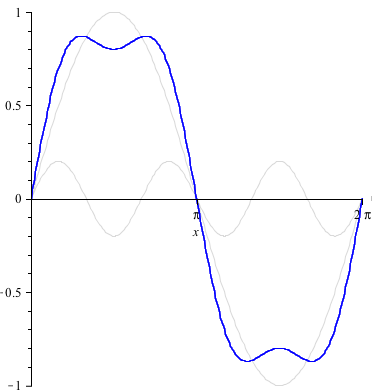
\includegraphics[scale=.4]{valg_af_loesning/thd/thdsamlet.png}
\caption{Eksempel på harmonisk forvrængning}
\label{fig:harmonic_distortion}
\end{figure}